\documentclass{report}
\usepackage{afterpage}
\usepackage{fullpage}
\usepackage{paralist}



% The following is needed in order to make the code compatible
% with both latex/dvips and pdflatex.
\ifx\pdftexversion\undefined
\usepackage[dvips]{graphicx}
\else
\usepackage[pdftex]{graphicx}
\DeclareGraphicsRule{*}{mps}{*}{}
\fi

\usepackage{tikz}
\usepackage[underline=true,rounded corners=false]{pgf-umlsd}
\usetikzlibrary{arrows,shadows} % for pgf-umlsd
\usepackage{tikz-er2} 

\newcommand{\MVCSlice}[1]{
\begin{figure}[htp]
\centering
\begin{tikzpicture}[shape aspect=.5, node distance=3cm, scale=0.5] 
%  \tikzset{every node/.style={draw}} 
  \tikzstyle{database} = [cylinder,shape aspect=.5, shape border rotate=90, minimum width=6cm, minimum height=1.5cm, draw] 
  \tikzstyle{layer} = [rectangle, minimum width=7cm, minimum height=2cm, draw]
  \tikzstyle{user} = [rectangle, minimum width=7cm, minimum height=1cm, draw]
  \tikzstyle{layer_annotation} = [rotate=90, node distance=3.75cm]
  \tikzstyle{line} = [<->, thick, shorten >=3pt, shorten <=3pt]
  \tikzstyle{mvc} = [rectangle, minimum width=2cm, minimum height=1cm, draw]
  \tikzstyle{mvc_left} = [mvc, anchor=east]
  \tikzstyle{mvc_right} = [mvc, anchor=west]
  \node [user] (user) {User};
  \node [layer, below of=user] (presentation_layer) {} node [layer_annotation,above of=presentation_layer] {Presentation Layer};
  \draw [line] (user) -- (presentation_layer);
  \node [layer, below of=presentation_layer] (business_layer) {} node [layer_annotation,above of=business_layer] {Business Layer};
  \node [layer, below of=business_layer] (data_layer) {} node [layer_annotation,above of=data_layer] {Data Layer};
  \node [database, below of=data_layer] (database) {DB};
  \draw (presentation_layer) node [mvc_left] (view) {#1 View};
  \draw (business_layer) node [mvc_right] (controller) {#1 Ctrlr};
  \draw (data_layer) node [mvc_left] (model) {#1 Model};
  \draw [line] (view) -- (model);
  \draw [line] (view) -- (controller);
  \draw [line] (controller) -- (model);
  \draw [line] (model) -- (database);
\end{tikzpicture}
\end{figure}
}

% Alter some LaTeX defaults for better treatment of figures:
    % See p.105 of "TeX Unbound" for suggested values.
    % See pp. 199-200 of Lamport's "LaTeX" book for details.
    %   General parameters, for ALL pages:
    \renewcommand{\topfraction}{0.9}	% max fraction of floats at top
    \renewcommand{\bottomfraction}{0.8}	% max fraction of floats at bottom
    %   Parameters for TEXT pages (not float pages):
    \setcounter{topnumber}{2}
    \setcounter{bottomnumber}{2}
    \setcounter{totalnumber}{4}     % 2 may work better
    \setcounter{dbltopnumber}{2}    % for 2-column pages
    \renewcommand{\dbltopfraction}{0.9}	% fit big float above 2-col. text
    \renewcommand{\textfraction}{0.07}	% allow minimal text w. figs
    %   Parameters for FLOAT pages (not text pages):
    \renewcommand{\floatpagefraction}{0.7}	% require fuller float pages
	% N.B.: floatpagefraction MUST be less than topfraction !!
    \renewcommand{\dblfloatpagefraction}{0.7}	% require fuller float pages

	% remember to use [htp] or [htpb] for placement




\newcommand{\CRUDcreate}[2]{
  \begin{sequencediagram}
    \newthread{browser}{:Browser}
    \newinst{controller}{:#1 Controller}
    \newinst{model}{:#1 Model}
    \newinst{data}{:MySQL}
    
    \begin{call}{browser}{GET '#2s/new'}{controller}{HTML/JavaScript}
      \begin{call}{controller}{new()}{model}{#1 > Active Record}
      \end{call}
    \end{call}
    \begin{call}{browser}{POST '#2s/new'}{controller}{HTML/JavaScript}
      \begin{call}{controller}{save()}{model}{true}
        \begin{callself}{model}{validate()}{true}
        \end{callself}
        \begin{call}{model}{INSERT}{data}{success}
        \end{call}             
      \end{call}
    \end{call}
  \end{sequencediagram}
}
\newcommand{\CRUDshow}[2]{
  \begin{sequencediagram}
    \newthread{browser}{:Browser}
    \newinst{controller}{:#1 Controller}
    \newinst{model}{:#1 Model}
    \newinst{data}{:MySQL}
    
    \begin{call}{browser}{GET '#2s/:id'}{controller}{HTML/JavaScript}
      \begin{call}{controller}{find(:id)}{model}{#1 > Active Record}
        \begin{call}{model}{SELECT}{data}{record}
        \end{call}
      \end{call}
    \end{call}
  \end{sequencediagram}
}
\newcommand{\CRUDlist}[2]{
  \begin{sequencediagram}
    \newthread{browser}{:Browser}
    \newinst{controller}{:#1 Controller}
    \newinst{model}{:#1 Model}
    \newinst{data}{:MySQL}
    
    \begin{call}{browser}{GET '#2s'}{controller}{HTML/JavaScript}
      \begin{call}{controller}{find(:all)}{model}{#1 > Active Record}
        \begin{call}{model}{SELECT}{data}{record}
        \end{call}
      \end{call}
    \end{call}
  \end{sequencediagram}
}
\newcommand{\CRUDupdate}[3]{
  \begin{sequencediagram}
    \newthread{browser}{:Browser}
    \newinst{controller}{:#1 Controller}
    \newinst{model}{:#1 Model}
    \newinst{data}{:MySQL}
    
    \begin{call}{browser}{GET '#2s/:id'}{controller}{HTML/JavaScript}
      \begin{call}{controller}{find(:id)}{model}{#1 > Active Record}
        \begin{call}{model}{SELECT}{data}{record}
        \end{call}
      \end{call}
    \end{call}
    \begin{call}{browser}{PUT '#2s/:id'}{controller}{HTML/JavaScript}
     \begin{call}{controller}{find(:id)}{model}{#1 > Active Record}
        \begin{call}{model}{SELECT}{data}{record}
        \end{call}
     \end{call}
     \begin{call}{controller}{update\_attributes(:#2)}{model}{success} 
        \begin{callself}{model}{validate()}{true}
        \end{callself}
        \begin{call}{model}{UPDATE}{data}{success}
        \end{call}        
     \end{call}
    \end{call}
  \end{sequencediagram}
}
\newcommand{\CRUDdelete}[2]{
  \begin{sequencediagram}
    \newthread{browser}{:Browser}
    \newinst{controller}{:#1 Controller}
    \newinst{model}{:#1 Model}
    \newinst{data}{:MySQL}
    
    \begin{call}{browser}{DELETE '#2s/:id'}{controller}{HTML/JavaScript}
      \begin{call}{controller}{find(:id)}{model}{#1 > Active Record}
        \begin{call}{model}{SELECT}{data}{record}
        \end{call}
      \end{call}
      \begin{call}{controller}{destroy()}{model}{true}
        \begin{call}{model}{DELETE}{data}{success}
        \end{call}
      \end{call}
    \end{call}
  \end{sequencediagram}
}
\newcommand{\CRUD}[2]{
\CRUDcreate{#1}{#2}
\CRUDshow{#1}{#2}
\CRUDlist{#1}{#2}
\CRUDupdate{#1}{#2}{Update a #1}
\CRUDdelete{#1}{#2}

}




\title{Software Design Description for Mashbot} 

\author{George D'Andrea \and Andrew Gall \and Josiah Kiehl \and
  Cody Ray \and Vito Salerno}
\date{\today}

\begin{document}

\begin{titlepage}
\maketitle
\end{titlepage}


\chapter*{Revision History}
\begin{tabular}{|p{2in}|l|l|l|}
  \hline
  \textbf{Name} & \textbf{Date} & \textbf{Reason for Changes} & \textbf{Version} \\
  \hline \hline
  George D'Andrea, Andrew Gall, Josiah Kiehl, Cody Ray, Vito
  Salerno & 17 January 2010 & Initial Version & 1.0 \\
  \hline
\end{tabular}

\clearpage
\tableofcontents
\clearpage

\chapter{Introduction}
\section{Purpose}
This document serves to expand upon the requirements document into implementation details and technology choices.  This document should be referenced when specific features are being implemented.
\section{Scope}
This covers the general architecture of Mashbot, as well as the design decisions used to apply that architecture via various appropriate technologies, libraries and frameworks.
\section{Definitions, Acronyms,   and Abbreviations}
\begin{itemize}
\item API | Application Programmming Interface
\item CRUD | Create Read Update Delete
\item CSS | Cascading Style Sheets
\item HAML | XHTML Abstraction Markup Language
\item MVC | Model View Controller
\item SASS | Syntactically Awesome Style Sheets
\item XHTML | Extensible Hypertext Markup Language
\end{itemize}
\section{Context Diagram}
\chapter{Architecture}
\section{Overview}
Mashbot will be implemented using a strict Model-View-Controller architecture.  This is augmented by the inclusion of the Publishing and Aggregation Platform, the purpose of which is to abstract the interaction with external service APIs from the application as a whole, thus allowing a pure MVC architecture to be implemented, increasing maintainability, flexibility and extensibility.
\section{Architecture}
\begin{itemize}
\item Campaign Manager
\begin{itemize}
\item Data Layer / Model
\item Presentation Layer / View
\item Business Layer / Controller
\end{itemize}
\item Campaign Workers
\item Publishing and Aggregation Platform
\end{itemize}
\section{Service-Oriented Architecture}
Mashbot will be implemented as two distinct yet related services.  The Campaign Manager will handle the interaction between the user and the data the Campaign Manager is concerned with, where the Publishing and Aggregation Platform will handle the interaction between external service APIs and the Campaign Manager.
\section{Survey of Technologies Used}
\subsection{Campaign Manager}
\begin{itemize}
\item Presentation Layer
  \begin{itemize}
  \item HAML | HTML replacement markup language, for building web layout structure.
  \item SASS | CSS replacement stylesheets, for applying visual styles to the layout built in HAML.
  \item jQuery | JavaScript library which provides cross-browser compatibility as well as streamlined Ajax request handling.
  \item Google Chart API | Public service provided by Google which generates many different kinds of charts and graphs.
  \end{itemize}
\item Business Layer
  \begin{itemize}
  \item Ruby | Dynamic programming language.
  \item Rails | Web application framework written in Ruby which provides a concise Model-View-Controller architecture.
  \item Heroku | Rails engine which provides enhanced production deployment via Rails compilation, a fast readonly filesystem, and horizontal scaling.
  \end{itemize}
\item Data Layer
  \begin{itemize}
  \item ActiveRecord | Component of Rails which provides the Active Record pattern of data access, creating data model objects and relationships for interacting with resources in a database.
  \item MySQL | Fast and free relational database which plugs into Rails without effort.
  \end{itemize}
\end{itemize}
\subsection{Publishing and Aggregation Platform}
\begin{itemize}
	\item Web Service Framework - Spring MVC. We chose this platform because
it offers a high degree configurable with zero code change. Important
options like defaults and the order of handlers on receiving a request is
completely configurable in XML.
\end{itemize}
\section{Presentation Layer Components}
\subsection{Campaign Views}
Campaigns are accessed via the Create and Manage tabs on the primary navigation tabs.  Create is for the Create view, Manage is for List, Show and Edit.
\clearpage
\begin{itemize}
\item Create | This is where users can create new campaigns.\\*
  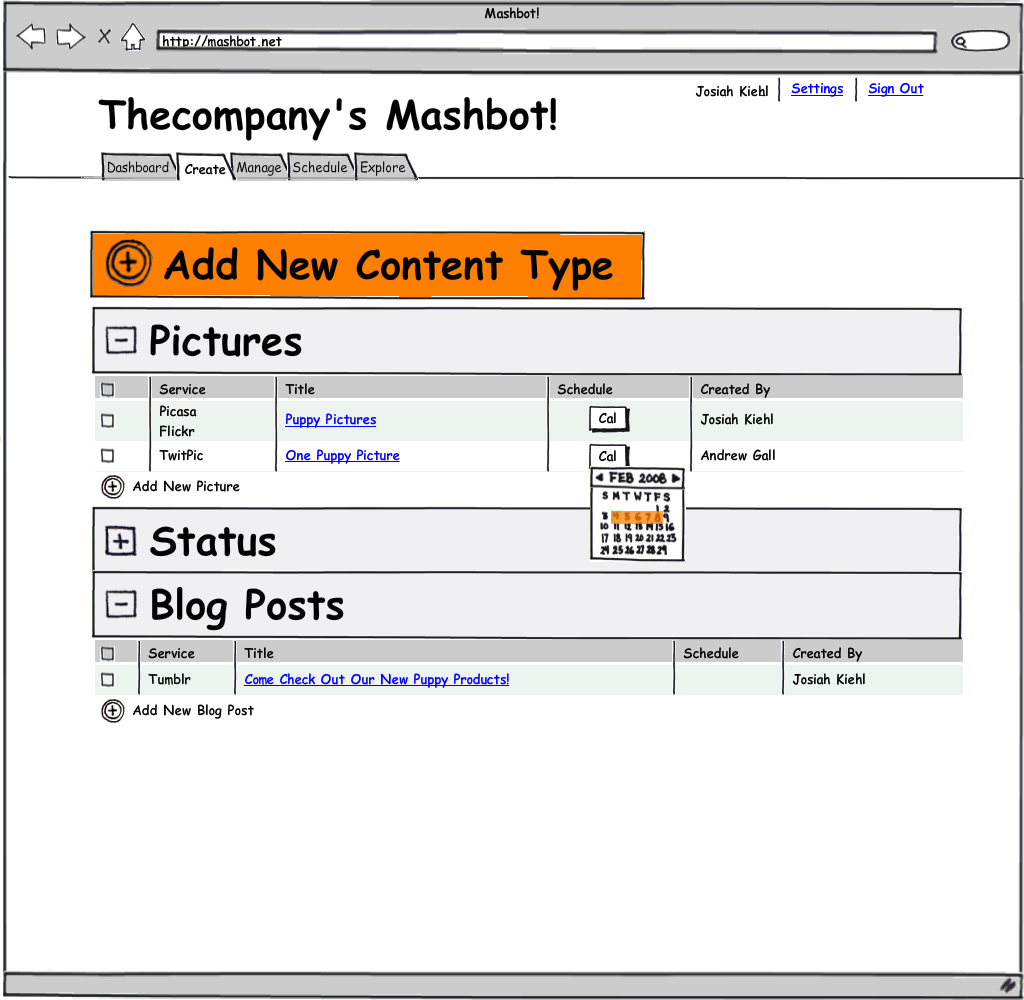
\includegraphics[width=\textwidth]{../mockups/create.png}
\item List | This is where users can view, update or delete existing campaigns. \\*
  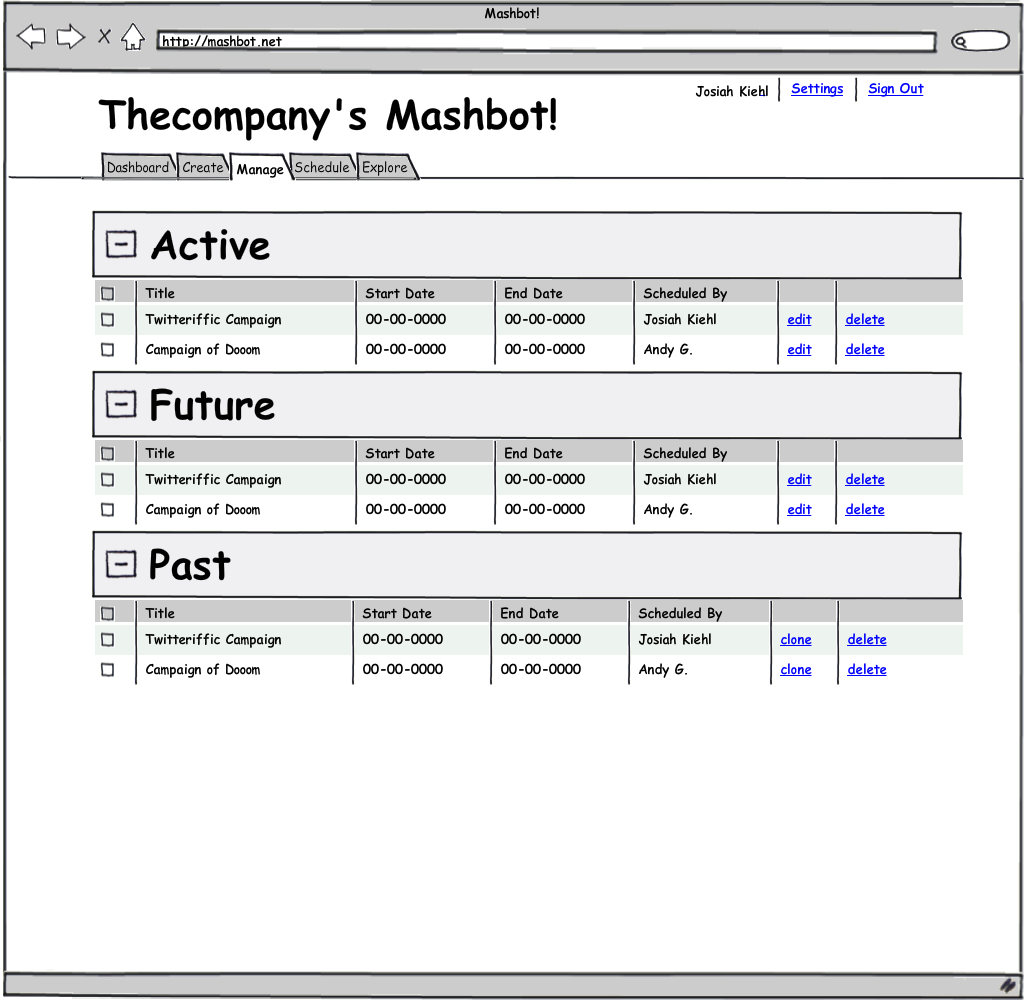
\includegraphics[width=\textwidth]{../mockups/manage.png}
\item Show | This view is what is shown when the user wants to view an existing campaign via the Show view.  This is also where the Content pieces will be listed. \\*
  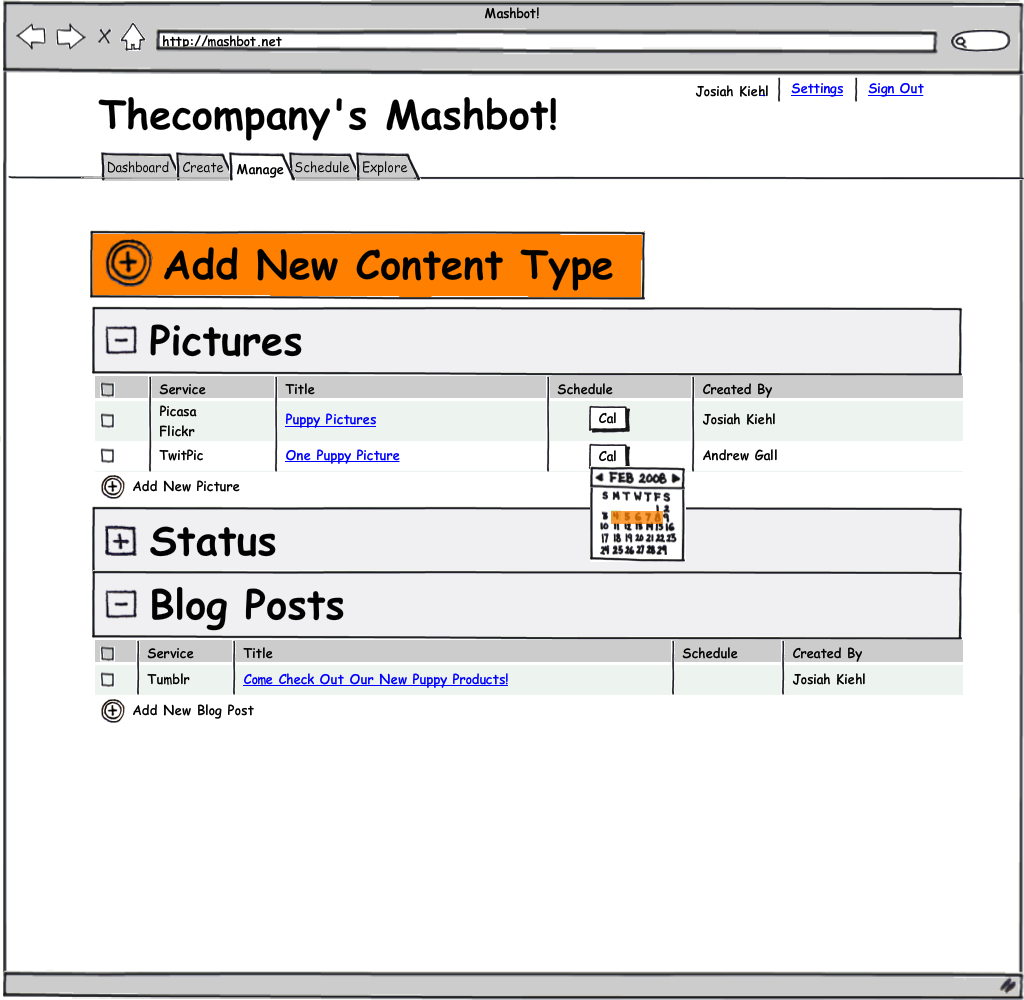
\includegraphics[width=\textwidth]{../mockups/manage-addcontent.png}
\item Edit | This is virtually the same view as Create, however this will be prepopulated with the existing content of the given Campaign.
\end{itemize}
\subsection{Content Views}
Content pieces are included inside Campaigns.  These views are accessible via the Show view of a Campaign for the corresponding Campaign id.
\begin{itemize}
\item Create | When on the Show view of a given campaign, the user can enter the Create view for Content.
\item Show | This is how the user previews the Content they have created.
\item Edit | This is virtually the same view as Create, however this will be prepopulated with the existing content of the given Content.
\end{itemize}
\subsection{Scheduling Views}
\begin{itemize}
  \item Primary Scheduling View |  consists of a list of Campaigns available to be scheduled (ie: they do not have existing start/stop dates) as well as already scheduled Campaigns placed properly on the calendar. \\*
  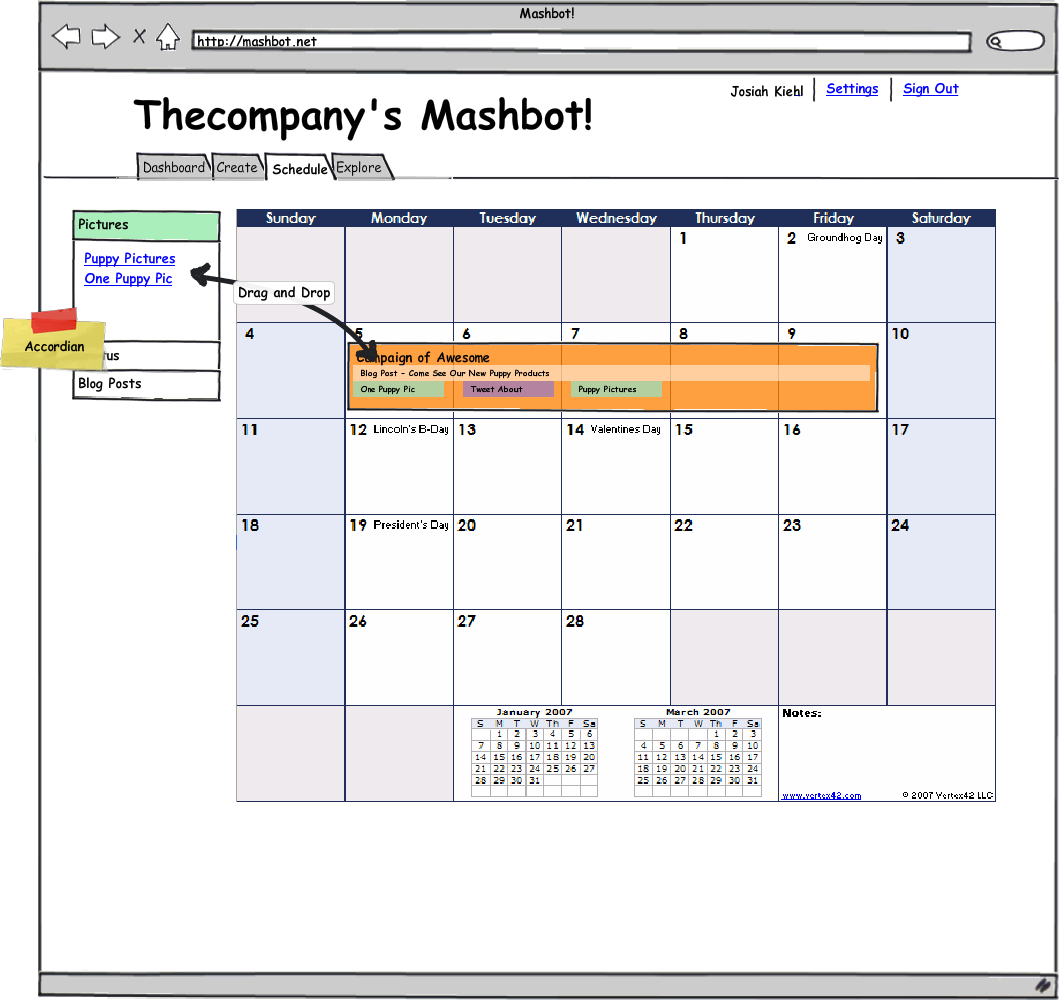
\includegraphics[width=\textwidth]{../mockups/schedule.png}
  \item Content Scheduling View | similar to the Primary Scheduling View, however the items available to be scheduled here are the individual content pieces of the Campaign.  This is accessed via selecting the Campaign from the calendar, or via the List Campaign or Show Campaign views. \\*
  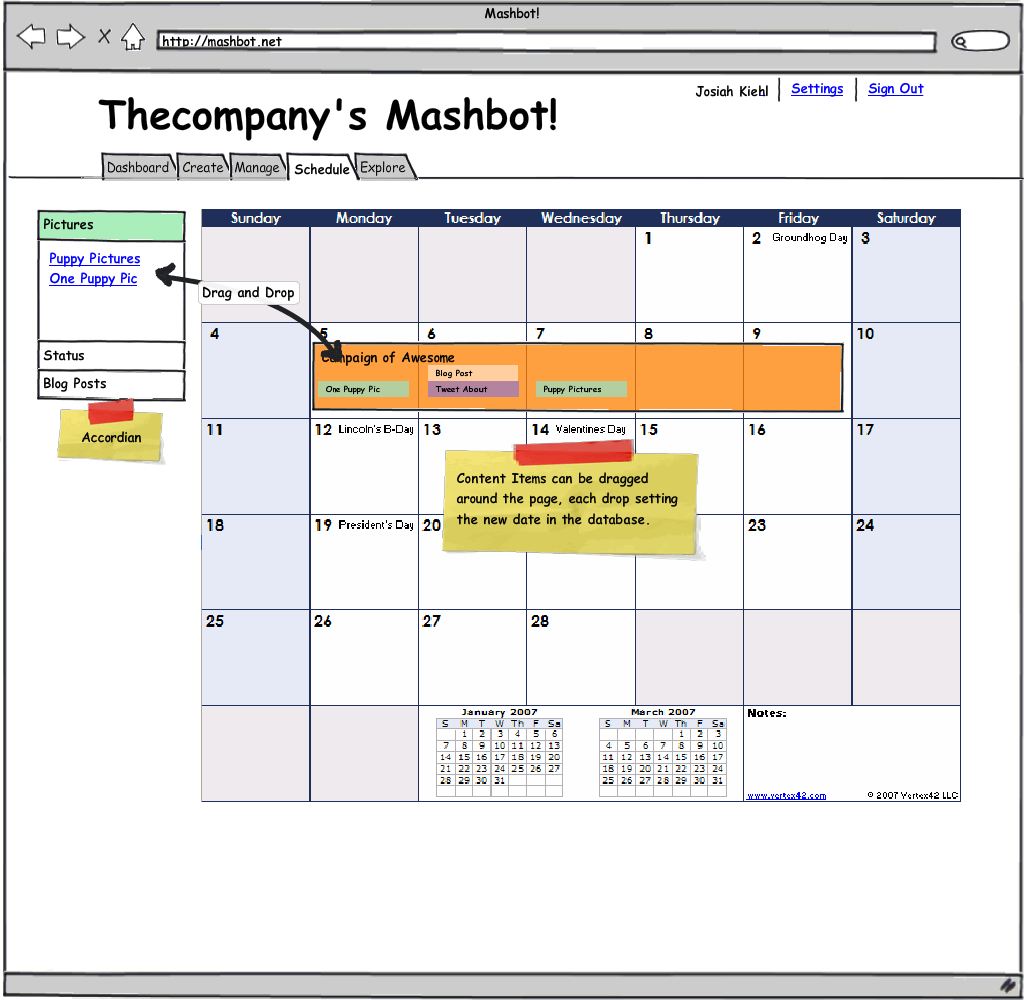
\includegraphics[width=\textwidth]{../mockups/schedule-content.png}
\end{itemize}
\subsection{Explore View}
 Here the user will have several available ``Insight Views.''  These are dependent on which plugins exist in the Publishing and Aggregation Platform, however there will be some provided by the Campaign Manager alone.  These will provide charts that are layerable, such that multiple charts can be seen on the same graph. \\*
  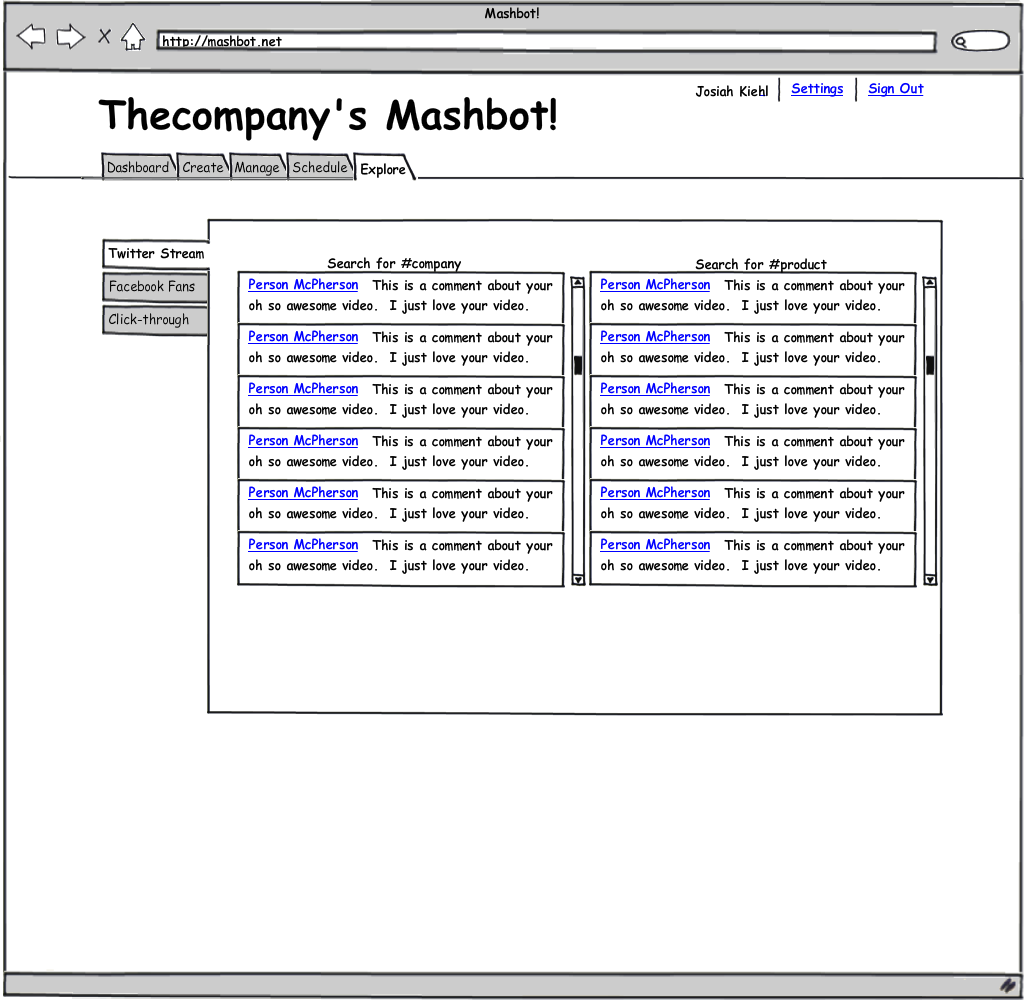
\includegraphics[width=\textwidth]{../mockups/explore-twitter.png}
\begin{itemize}
\item Plugin Independent
  \begin{itemize}
  \item Clickthrough tracking | Any time a link is generated via Mashbot, it is given a special redirecting URL that will allow Mashbot to track how many times the link has been clicked.
  \item Rate of publishing | How often does the user tweet/blog/etc. This will most likely be used to correlate frequency with user engagement.
  \end{itemize}
\item Plugin Dependent
  \begin{itemize}
  \item Facebook Fan tracking | A line chart of how many fans the user's fan page has. \\*
    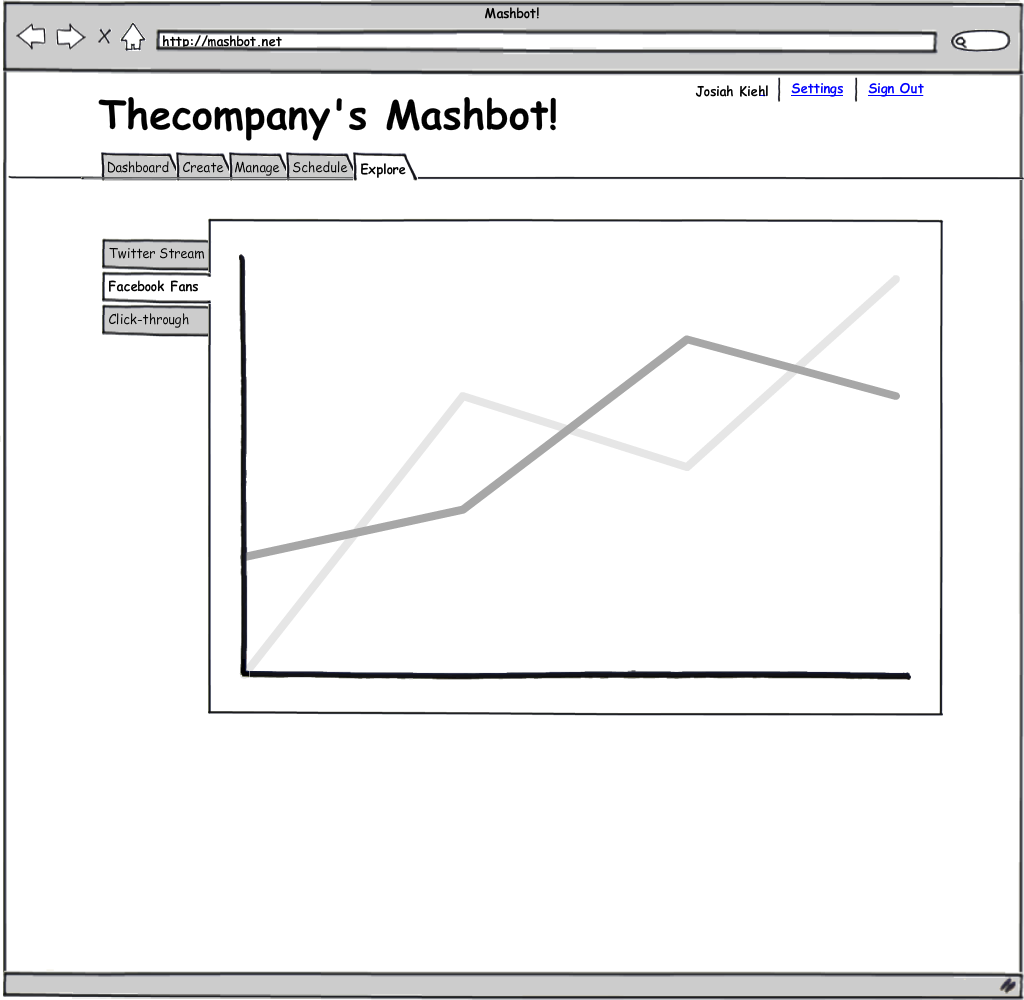
\includegraphics[width=\textwidth]{../mockups/explore-facebook.png}
  \item Twitter Follower tracking | A line chart of the number of twitter followers the user's Twitter account has.
  \item Number of times retweeted | A line chart of the number of times a tweet of the user's has been retweeted.
  \end{itemize}
\end{itemize}

\section{Business Layer Components}
\subsection{Session and Authentication}

At the user layer, the authentication engine will use a secure password / token based system. In addition to the default username/password option, Mashbot will also support login through OpenID, Facebook Connect, and Twitter/OAuth.

The Mashbot authentication system will provide three different kinds of security tokens that tasks may need, rather than providing users with a token for each task (reset passwords, etc.). The tokens are the ``keys'' to do the following:
\begin{itemize}
\item Persistence token: Used internally, it is stored in your cookies and sessions to persist the user. This is much more secure than plainly storing the user�s id.
\item Single access token: Use this for a private feed or API access. For example,\\
          \texttt{www.example.com?user\_credentials=[single access token]} grants access but does NOT persist.
\item Perishable token: Great for authenticating users to reset passwords, confirm their account, etc.
\end{itemize}

Additionally, all cryptographic routines will be provided by external, third-party verified modules to ensure that their implementation is correct and secure. The authentication framework itself will be largely provided by a widely-used open source Ruby library known as authlogic.

\subsubsection{Log In}

For password-based authentication, the password will be processed through a one-way hash function (SHA512 by default) and only the hashed password will be stored in the database. This mechanism avoids the potential of password recovery if the database becomes compromised.

\MVCSlice{User Session}
  \begin{sequencediagram}
    \newthread{browser}{:Browser}
    \newinst{controller}{:Controller}
    \newinst{model}{:User Session Model}
    \newinst{data}{:MySQL}
    \begin{call}{browser}{HTTP POST}{controller}{}
      \begin{call}{controller}{Authenticate()}{model}{}
        \begin{call}{model}{SELECT}{data}{}
        \end{call}
      \end{call}
    \end{call}
  \end{sequencediagram}

\subsubsection{Log Out}

During the logout process, the session is destroyed. Both the session cookies and the corresponding server-side hash fingerprint are erased.

  \begin{sequencediagram}
    \newthread{browser}{:Browser}
    \newinst{controller}{:Controller}
    \newinst{model}{:User Session Model}
    \newinst{data}{:MySQL}
    \begin{call}{browser}{HTTP POST}{controller}{HTML/JavaScript}
      \begin{call}{controller}{log\_out}{model}{true}
        \begin{call}{model}{UPDATE}{data}{success}
        \end{call}
      \end{call}
    \end{call}
  \end{sequencediagram}

\subsubsection{OAuth}

At the API layer, Mashbot will use the OAuth standard. OAuth is an open protocol to allow secure API authorization in a simple and standard method from desktop and web applications. OAuth allows users to share their private resources (e.g. photos, videos, contact lists) stored on one site with another site without having to hand out their username and password. OAuth allows users to hand out tokens instead of usernames and passwords to their data hosted by a given service provider. Each token grants access to a specific site (e.g. a video editing site) for specific resources (e.g. just videos from a specific album) and for a defined duration (e.g. the next 2 hours). Thus OAuth allows a user to grant a third party site access to their information stored with another service provider, without sharing their access permissions or the full extent of their data.

\subsubsection{OpenID}

OpenID is an open, decentralized standard for authenticating users which can be used for access control, allowing users to log on to different services with the same digital identity where these services trust the authentication body. OpenID can replace the common login process that uses a login-name and a password, by allowing a user to log in once and gain access to the resources of multiple software systems

\subsubsection{Session Handling}

Mashbot uses a cookie-based session store and avoids storing confidential information in its session. In order to prevent attacks by client-side cookie modification, sessions have a SHA512 fingerprint attached and are hashed with a secret stored on the server. Using a cookie-based session increases performance, avoids the ``server stickiness'' issue associated with horizontal scaling, and increases performance due to an avoided database query on every page load.

\section{Data Layer Components}
\subsection{ActiveRecord}
ActiveRecord is a library which maps database tables to objects. It allows the columns of tables to be accessed as attributes of a Ruby object. Additionally, it handles all of the relationships between tables as well as validation for input.
\subsection{MySQL}
MySQL is a fast, free relational database management system solution.
\section{External Components}
\subsection{Publishing and Aggregation Targets}
\begin{itemize}
\item Flickr
\item Picasa
\item Twitter
\item Tumblr
\item Wordpress
\item YouTube
\end{itemize}
\subsection{Email/SMTP Service}
Email will be used to notify users of reset lost usernames and passwords.
  \begin{sequencediagram}
    \newthread{manager}{:Campaign Manager}
    \newinst{daemon}{:Delayed Job Daemon}
    \newinst{mailer}{:Mailer Worker}
    \newinst{mail}{:SMTP Server}
    \begin{call}{manager}{send\_later()}{daemon}{true}
    \end{call}
    \begin{callself}{daemon}{act()}{true}
        \begin{call}{daemon}{perform}{mailer}{true}
          \begin{call}{mailer}{sendmail()}{mail}{true}
          \end{call}
        \end{call}
    \end{callself}
  \end{sequencediagram}

\section{External Authentication via OpenID}

\MVCSlice{OAuth}
  \begin{sequencediagram}
    \newthread{browser}{:Browser}
    \newinst{controller}{:OAuth Controller}
    \newinst{model}{:Authentication Model}
    \newinst{data}{:MySQL}
    \newinst{external}{:External Authentication API}
    \begin{call}{browser}{HTTP POST}{controller}{HTML/JavaScript}
      \begin{call}{controller}{Authenticate()}{model}{true}
        \begin{call}{model}{SELECT}{data}{record}
        \end{call}
      \end{call}
    \end{call}
  \end{sequencediagram}
  \begin{sequencediagram}
    \newthread{browser}{:Browser}
    \newinst{controller}{:OAuth Controller}
    \newinst{model}{:Authentication Model}
    \newinst{data}{:MySQL}
    \newinst{external}{:External Authentication API}
    \begin{call}{browser}{HTTP POST}{controller}{HTML/JavaScript}
      \begin{call}{controller}{Authenticate()}{model}{true}
        \begin{call}{model}{SELECT}{data}{record}
        \end{call}
        \begin{call}{model}{Authenticate()}{external}{true}
        \end{call}
      \end{call}
    \end{call}
  \end{sequencediagram}

\section{User Accounts}
\subsection{Create User Account}
This is a basic CRUD operation: Create User Account. \\*
\CRUDcreate{User Account}{user}
\subsection{Update User Account}
This is a basic CRUD operation: Update User Account. \\*
\CRUDupdate{User Account}{user}{Update a User Account}
\subsection{Delete User Account}
This is a basic CRUD operation: Delete User Account. \\*
\CRUDdelete{User Account}{user}
\section{Campaigns}
\MVCSlice{Campaign}
\subsection{Create Campaign}
This is a basic CRUD operation: Create Campaign. \\*
\CRUDcreate{Campaign}{campaign}
\subsection{View Campaign}
This is a basic CRUD operation: View Campaign. \\*
\CRUDlist{Campaign}{campaign}
This is a Read operation, similar to the above, but for one Campaign. \\*
\CRUDshow{Campaign}{campaign}
\subsection{Update Campaign}
This is a basic CRUD operation: Update Campaign. \\*
\CRUDupdate{Campaign}{campaign}{Update a Campaign}
\subsection{Delete Campaign}
This is a basic CRUD operation: Delete Campaign. \\*
\CRUDdelete{Campaign}{campaign}
\subsection{Schedule Campaign}
This is a basic CRUD operation: Schedule Campaign. \\*

\CRUDupdate{Schedulable Unit}{schedulable\_unit}{Update scheduled time of Schdulable Unit}
\section{Content Units}
\subsection{Create Content Unit}

\MVCSlice{Content Unit}
This is a basic CRUD operation: Create Content. \\*
\CRUDcreate{Content Unit}{content\_unit}
\subsection{View Content Unit}
This is a basic CRUD operation: View Content\_Unit. \\*
\CRUDlist{Content Unit}{content\_unit}
This is a Read operation, similar to the above, but for one Content Unit.  \\*
\CRUDshow{Content Unit}{content\_unit}
\subsection{Update Content Unit}
This is a basic CRUD operation: Update Content\_Unit. \\*
\CRUDupdate{Content Unit}{content\_unit}{Update content\_unit}
\subsection{Delete Content Unit}
This is a basic CRUD operation: Delete Content\_Unit. \\*
\CRUDdelete{Content Unit}{content\_unit}
\subsection{Schedule Content Unit}
In order to change the scheduled time of anything that is schedulable, the same process as an update is carried out. \\*
\CRUDupdate{Schedulable Unit}{schedulable\_unit}{Update scheduled time of a Schedulable Unit}

After content is scheduled, it can be picked up by the Scheduler, triggered via Cron.  Every 30 minutes, Cron will run the Scheduler, which will look in the database for active Campaigns.  Within those active campaigns, each piece of content will be checked to see if the go-live time is now or past.  If it's now or past, the scheduler calls the Publishing and Aggregation Platform with the content needed for a push to the given External Service.
  \begin{sequencediagram}
    \newthread{cron}{:Cron}
    \newinst{scheduler}{:Scheduler}
    \newinst{worker}{:Worker}
    \newinst{data}{:Database}
    \begin{call}{cron}{cron trigger}{scheduler}{exit 0}
      \begin{callself}{scheduler}{anything\_to\_do?()}{true}
        \begin{call}{scheduler}{SELECT}{data}{record}
        \end{call}
      \end{callself}
      \begin{call}{scheduler}{perform()}{worker}{true}
      \end{call}
    \end{call}
\end{sequencediagram}
\section{View Metrics and Statistics via Explore Panel}
\section{Lost User Name}
\MVCSlice{User Account}
  \begin{sequencediagram}
    \newthread{browser}{:Browser}
    \newinst{controller}{:User Account Controller}
    \newinst{model}{:User Account Model}
    \newinst{data}{:MySQL}
    \begin{call}{browser}{HTTP POST}{controller}{HTML/JavaScript}
      \begin{call}{controller}{find\_by\_email(email)}{model}{User > Active Record}
        \begin{call}{model}{SELECT}{data}{record}
        \end{call}
      \end{call}
    \end{call}
  \end{sequencediagram}
\section{Lost Password}
  \begin{sequencediagram}
    \newthread{browser}{:Browser}
    \newinst{controller}{:User Account Controller}
    \newinst{model}{:User Account Model}
    \newinst{data}{:MySQL}
    \newinst{mailer}{:Mailer}
    \begin{call}{browser}{HTTP POST}{controller}{HTML/JavaScript}
      \begin{call}{controller}{reset\_password()}{model}{true}
        \begin{call}{model}{UPDATE}{data}{success}
        \end{call}
        \begin{call}{model}{sendmail()}{mailer}{true}
        \end{call}
      \end{call}
    \end{call}
  \end{sequencediagram}
\chapter{Publishing and Aggregation Platform}
	\section{Object Model}
		\subsection{Overview}
			Objects exist in Mashbot for the purposes of identification and 
			manipulation. Objects are not stored in the Publishing and 
			Aggregation Platform, but are merely passed through its pipeline.

			Objects contain information general to that object itself and also 
			information specific to one or more services, so as to
			identify that object on a service, or distinguish similar fields in 
			different services.

			Each object has a type and comprises two collections of entities:
			(1) a set of service associations, and (2) a list of properties in 
			the form of a collection of objects.  An object can also be 
			considered ``primitive,'' meaning it has an unstructured value 
			assigned to it.

			Semantically speaking, an object is anything that can be 
			manipulated by people and computers in a web context.  Examples of 
			objects are pictures, blog posts, status updates, IDs, people, et 
			al.  Not all of these are supported by Mashbot initially, but could 
			be added through the plugin architecture.

		\subsection{The Object}
			The object comprises:
			\begin{itemize}
			\item Type
			\item Service Associations
			\item Properties
			\item \emph{(Optionally)} Primitive value
			\end{itemize}

		\subsubsection{Type}
			An object has type associated with it. Type is service agnostic:
			multiple services may support handling the same type of object,
			and services may support handling multiple object types.
		\subsubsection{Service Associations}
			Each object may be associated with one or more services.
			Semantically, this reflects the idea that an object, as 
			manipulated by Mashbot, exists in parallel with an object stored in 
			some form on each associated service.

			That is to say, an object associated with a particular service is 
			``live'' on that particular service, and an object not associated 
			with any service is ``not live,'' and does not exist on that 
			service.

			Associations tell the Publishing and Aggregation Platform where to 
			look for an object, that is, which plugins to use to index and pull 
			a given object.

			\textbf{Adding/removing an association}:
			Adding an assocation is ``pushing'' an object to that service.  
			Removing an association is ``deleting'' an object from that
			service.  
			
			These operations are defined by plugins in terms of both
			\emph{behavior} and \emph{requirements}. Requirements may be
			complex and hierarchical, specifying recursive requirements for 
			values and sub-objects within a given object.			
		\subsubsection{Properties}
			Properties represent an unordered collection of child objects 
			belonging to the object in question. Child objects are not mandated to be of a unique type or value, and 
			thus cannot be addressed by type or value. Instead, objects can be 
			queried for child objects, given criteria about the child objects 
			themselves.

			For instance, an object may be associated with two different 
			services, and thus have two different identifiers. That object, 
			therefore, will have one child object ID associated with the first 
			service, and a second child object ID associated with the second 
service. (But the numbering here is arbitrary)

			This isn't to say that child objects cannot be associated with more 
			than one service. The demarcation again is semantic: if two 
			entities refer to the same thing, they should be the same object.
			For instance, an object that has a name might have the same name on 
			two different services, so the object would have a single child 
			object for name, and both objects would be associated with both 
			services.

		\subsubsection{Primitive value} 

			A primitive value is a value with which the object can be 
			interchanged without losing or gaining semantic information.

			For instance, IDs and names are object types that would frequently 
			have primitive values. An ID could have a primitive value 
			\emph{1000}, and a name could have a primitive value \emph{Bob's 
			  Photo}.
		\subsection{Class Diagram}
			\includegraphics{uml/object_model.1}
    \subsection{Sequence Diagram}
      \subsubsection{Pushing to a Service}
      \begin{sequencediagram}
      \newthread{obj}{Object}
      
      \newinst[1]{req}{Service Requirements}
      \newinst{svc}{Service Request}

      \begin{call}{obj}{checkRequirements(this)}{req}{}
      \end{call}

      \begin{call}{obj}{push(this)}{svc}{response}
        \begin{call}{svc}{addProperties(newProperties)}{obj}{}
        \end{call}
        \begin{call}{svc}{addAssociation(serviceAssociation)}{obj}{}
        \end{call}
      \end{call}

      \end{sequencediagram}


	
	\section{API Design}
		\subsection{Request}
			A request to our API will have the following fields:
			\begin{itemize}
				\item OAuth Information
					\begin{itemize}
						\item Realm - A Protection Realm
						\item Consumer Key - A key for identifying the customer
						\item Access Token - A token generated using the
					   	parameters and the Consumer Secret
						\item Nonce - A randomly generated string given to all
					   	requests sent with the same timestamp.  
						\item Timestamp - The number of seconds since January
					   	1st, 1970.
						\item Signature Method - The signature method that the
					   	user used to sign the request
						\item Version - Version of OAuth that you are using.
					\end{itemize}
				\item Operation - A string containing the operation as detailed 
				  below.
				\item Content - The content to be passed to the appropriate
					Content Processors. This contains all the information encompassed by 
					our Object Model.
				\item Third Party Authentication Data - The third party
				  authentication data for sending third party requests. It will
				  contain a tree whose hierarchy will contain the following
				  levels.
					\begin{enumerate}
						\item Service Name
						\item User Name
						\item Authentication - Contains either the
						  authentication token for this user or a password
					\end{enumerate}
			\end{itemize}
		\subsection{Operation}
			The operation is the type of action which you wish to perform on our 
			service. This partly defines what type of information is required in the 
			request. However, these fields are not inherent and in fact, the 
			information that is required in any request is defined by any plugin 
			which supports a given content type. The operation space is completely 
			unlimited but the four operations below are planned to be the main 
			operations supported by the Mashbot project. 
                        
                        \subsubsection{Push}
                                In this operation, the user will provide all the necessary information
                                for a piece of content to be posted to the services specified. 
                                Assuming success, they will be returned identifying information for
                                the content on each service.
			
			\subsubsection{Delete}
				In this operation, the user will provide identifying information for 
				items which they wish to be deleted from the services identified.
				
			\subsubsection{Edit}
				In this operation, the user will provide identifying information for 
				already posted material and an edited version of the original content 
				which the user wishes to be replaced on services for which information 
				has been provided.
			
			\subsubsection{Pull}
			        In this operation, the user will provide identifying information for a
                                previously posted piece of content which will be retrieved from the
                                specified services. In the case that the specified content is not
                                identical between the services, each unique piece of content will be
                                returned.

		\subsection{Content Types}
                        The content type determines what type of content we are performing an operation
                        on. Like operations, they partly define what information is required for a
                        request. Also like operations, the ones mentioned below are not the only ones
                        Mashbot will support. Any service plugin can define a new content type and
                        determine what fields are required for a successful post. We will also allow for
                        different ways of specifying the content. For example, a user may upload an image
                        and use that to post a picture. However, if a service supports it the user can
                        submit a URL pointing to a photo instead. The four main types of content we expect
                        to deal with are the following.

			\subsubsection{Blog Post}
			        A blog post will generally have two components, a title, and a body. Both
                                of these will be text fields, but the assumption is that users can embed
                                HTML if they would like more content rich posts.

			\subsubsection{Picture}	
                                A picture post's required components are expected to change a little
                                depending on the service to which it is posted. We expect most plugins
                                to require (or at least support) the actual image, a title, description,
                                and album to which the image should be posted.

			\subsubsection{Status}
                                A status is expected to be the simplest type of content. It only requires
                                a single text field, which is the status.

			\subsubsection{Video}
                                Video should have the same required fields as a picture, exchanging the
                                image for a video. A service may also require one or more preview image(s).

	\section{Server Design}
		\subsection{Platform}
			We plan to build this server on an existing web service framework. This 
			means that everything up until the point where execution and the incoming 
			request is passed to the handler chain when a request is made will be handled by this existing framework. Most 
			configuration will be carried in XML.
		
		\subsection{Architecture}
			The internal architecture follows the handler chain pattern. The 
			HandlerChain class holds a linked list of handlers. As demonstrated below:

                          \begin{sequencediagram}
                            \newthread{previousHandler}{:Previous Handler}
                            \newinst{currentHandler}{:Current Handler}
                            \newinst{nextHandler}{:Next Handler}
                            \begin{call}{previousHandler}{enact()}{currentHandler}{}
                            \begin{callself}{currentHandler}{preRequest()}{}
                            \end{callself}
                            \begin{call}{currentHandler}{enact()}{nextHandler}{}
                            \end{call}
                            \begin{callself}{currentHandler}{postRequest()}{}
                            \end{callself}
                            \end{call}
                          \end{sequencediagram}
		\subsection{HandlerChain}
			This class embodies the linked list that is
                        the handler chain. It will the pass 
			the request information to the first Handler and then that handler will 
			call each subsequent handler in the chain. This class will also
handle initializing the linked list itself as it will take as an argument an
arraylist of Handlers. It also unless to segregrate the functionality of
linking all of the Handlers together outside of the Handler classes instead
of hard coding into the code what the next handler will be for each. 
	
			\includegraphics{uml/HandlerChain.2}
		\subsection{Handlers}
			\subsubsection{Handler}
				This is an interface which describes what methods must be provided in 
				order for a class to be considered a handler. A Handler is a class which 
				can take in a request, perform some preprocessing, perform the actual 
				operations, and then perform post processing before returning have 
				made any necessary changes to the response.
				
				\includegraphics{uml/Handlers.1}
			\subsubsection{ChainableHandler}
				A chainable handler is one which can be placed in a sequence of handlers 
				with the knowledge of who is next in line. This means that it will 
				perform preprocessing and postprocessing, before and after calling the 
				next handler in the chain respectively.
				
				\includegraphics{uml/Handlers.2}
			\subsubsection{AuthenticationHandler}
				The authentication handler will take the authentication information from 
				the Request object and after having performed authentication of the user 
				will insert the unique user identifier into the Context object passed up 
				the Handler chain.

				\includegraphics{uml/Handlers.3}
			\subsubsection{SerializationHandler}
				The serialization handler extracts the raw data from the Content field 
				and creates a new Content object from that containing all the data. The 
				information contained in this is encompassed by the object model. See 
				the object model section for more information. It then places this 
				Content in the application context on its way in. On the way out, it 
				will take the Content object from the Context. Then, it will reserialize it and place it in the Response.

				\includegraphics{uml/Handlers.4}
			
			\subsubsection{RequiredDataVerificationHandler}
			This handler queries the plugins which handle the operation and content 
			type which has been specified by the request with the fields that are 
			present to make sure that all requisite data for that request is present.  
			If all required data for any one service is not present, the request fails 
			at this step. Otherwise, the request continues through the system.
				
			\includegraphics{uml/Handlers.5}
				
			\subsubsection{ContentProcessingHandler}
			This handler loops through and calls the plugins which correspond to
			the operation, the content type, and the services which have been 
			specified in the request passing them the content blob of the request. The 
			plugin will return the blob. All plugins must conform to the 
			ContentProcessor Interface.
			
			\includegraphics{uml/Handlers.6}


			\subsubsection{Overall}

			\includegraphics{uml/Handlers.7}

  \section{Sequence Diagram for Handling a Request}
    %\begin{figure}
    \begin{sequencediagram}
    \newthread{req}{Receiving}
    \newinst{auth}{Authentication}
    \newinst{serial}{Serialization}
    \newinst{ver}{Data Verification}
    \newinst{proc}{Content Processing}
    \newinst{svc}{Service Plugin}

    \begin{call}{req}{authenticate()}{auth}{}
      \begin{call}{auth}{build()}{serial}{}
        \begin{call}{serial}{verify()}{ver}{}
          \begin{call}{ver}{checkRequirements()}{svc}{}
          \end{call}
          \begin{call}{ver}{process()}{proc}{}
            \begin{call}{proc}{serviceRequest()}{svc}{}
            \end{call}
          \end{call}
        \end{call}
      \end{call}
    \end{call}


    \end{sequencediagram}
    %\caption{Sequence Diagram for Handling a Request} \end{figure}

			
	\section{Plugin Design}
		\subsection{I suck at life}
		\subsection{Service Plugins}
                        \subsubsection{Flickr}
                              The only thing the Flickr API requires for a photo upload is the
                              photo itself. Optional parameters include a title, description,
                              tags, and access control parameters. The API also allows user to
                              edit or delete photos and add photos to albums. We plan on
                              providing at least these functions.
                        \subsubsection{Picasa}
                              Picasa provides a similar API to Flickr, except we must provide
                              an explicit album for a picture to go into (although there is a
                              default album).
                        \subsubsection{Twitter}
                              The only real object we need to deal with in twitter are tweets
                              (status updates). Twitter allows for the posting of tweets and
                              deletion of tweets. It also offers the ability to retweet (copy
                              another user's tweet). We will provide access to all these
                              actions. Twitter also provides a number of API calls which will
                              be useful for our tools for analytics
                        \subsubsection{Tumblr}
                              Tumblr allows a variety of post types, which include ``regular,''
                              ``photo,'' ``quote,'' ``link,'' ``conversation,'' ``video,'' and
                              ``audio.'' Many of these post types contain fields that accept
                              HTML. We will support all these post types. Tumblr also provides
                              edit and delete API calls.
                        \subsubsection{Wordpress and Blogger}
                              Wordpress provides a variety of web APIs, but we will use the one
                              which is compatible with Blogger. It allows for posts with only
                              a title and content fields. The content field accepts HTML. It
                              also provides the ability to edit and delete posts.
                        \subsubsection{YouTube}
                              Youtube videos require a title, description, category and keywords
                              in addition to the actual video data. YouTube supports both direct
                              uploads and browser based uploads. Our plan is to only support
                              browser based uploads. YouTube also supports the modification
                              and deletion of videos, which we will support.
\chapter{Database Design}
\section{Summary}

An entity-relationship diagram depicting the data model is shown below, which uses the E-R notation described in the book Database System Concepts, by Silberchatz et al. 
% Should either remove some authn detail, or add some domain (campaign publishing) detail.

\tikzstyle{every relationship} = [fill=red!20] 
\tikzstyle{every edge} = [link] 
\begin{tikzpicture}[node distance=8em]
	\node[entity] (account) {Account}; 
	\node[relationship] (authenticates) [right of=account] {Authenticates} edge (account);
	\node[relationship] (has) [below  of=authenticates] {Has} edge (account);
	\node[entity, node distance=10em] (user) [right of=has] {User} edge (has);
	\node[entity] (service) [right of=authenticates] {Service} edge (authenticates);
	\node[entity] (campaign) [above of=account] {Campaign} edge [->] (account);
	\node[relationship] (publishes) [right of=campaign] {Publishes} edge (campaign);
	\node[entity] (content) [right of=publishes] {Content} edge (publishes);
	\node[entity, node distance=10em] (openid_ident) [below of=user] {OpenID Identifier} edge [->] (user);
	\node[entity, node distance=10em] (openid_assoc) [left of=openid_ident] {OpenID Association};
	\node[entity, node distance=9.5em] (openid_nonce) [left of=openid_assoc] {OpenID Nonce};
	\node[rectangle, draw=gray, fit=(openid_ident) (openid_assoc) (openid_nonce), inner sep=1em] {};
	\node[entity, node distance=10em] (client_application) [left of=account] {Client Application} edge (account);
	\node[entity] (oauth_provider_token) [above of=client_application] {OAuth Provider Token} edge [->] (client_application) edge [->] (account);
	\node[entity] (oauth_nonce) [above of=oauth_provider_token] {OAuth Nonce};
	\node[rectangle, draw=gray, fit=(client_application) (oauth_provider_token) (oauth_nonce), inner sep=1em] {};
	\node[entity] (oauth_consumer_token) [below of=client_application] {OAuth Consumer Token} edge (account);
	\node[rectangle, draw=gray, fit=(oauth_consumer_token), inner sep=1em] {};
\end{tikzpicture} 

\subsection{Advantages of Design}
\begin{itemize}
\item Decoupled Publishing Platform
  \begin{itemize}
  \item Allows publishing capabilities to be extended without change to the Campaign Manager.
  \item Provides asynchronous publishing so HTTP requests do not time out when pushing a large amount of content.
  \item Allows scheduled items to get fired off, even if the Campaign Manager is not fully running.
  \end{itemize}
\item Extensibility
  \begin{itemize}
    \item Easy to add support for new social media services
    \item Easy to add support for new content types
    \item Easy to add support for new operation types
  \end{itemize}
\item Request pipeline is easily modifiable
  \begin{itemize}
    \item Easy to add new authentication types
    \item Simple to add pre-processing steps
  \end{itemize}
\item 
\end{itemize}

\subsection{Disadvantages of Design}
\begin{itemize}
  \item Support for new content types will force additional development if generic file uploads are not sufficient to handle publishing the content.
  \item Generality of our design may create performance bottlenecks in the future
  \item We will be limited by the capabilities of the web service framework we choose.
  \item The campaign manager design presupposes a certain amount of familiarity with social media concepts
\end{itemize}
\section{Requirements Traceability Table}

\end{document}


% LocalWords:  Mashbot
